\chapter{Results}
\label{sec:results}

This chapter answers RQ4. Section~\ref{sec:r-saturation} measures saturation across
the suite, confirming the diagnosis of Section~\ref{sec:m-saturation}.
Section~\ref{sec:r-toy} isolates the estimator on a controlled toy.
Section~\ref{sec:r-anchors} reports the head-to-head on the systems where saturation
bites, and Section~\ref{sec:r-cross} on the systems where it does not.
Section~\ref{sec:r-ablation} is the ablation study: it separates the contribution of
the estimator from that of the optimiser. Section~\ref{sec:r-perstep} reads the
rollouts step by step and shows that performance is not predicted by the effective
sample size, and Section~\ref{sec:r-diag} reports the diagnostics that justify
trusting the method when that sample size is small.

All numbers are from the validated result set. Each main comparison uses $n=300$
paired rollouts, with the sPCE lower bound and sNMC upper bound on the same rollouts
at the same budget $L_{\mathrm{eval}}$. A dagger ($\dagger$) marks a definitive
ordering, where one method's lower bound exceeds the other's upper bound by more than
the combined standard error.

\section{Saturation across the suite}
\label{sec:r-saturation}

Figure~\ref{fig:lscan} shows the saturation transition for five representative
systems as the contrastive budget grows. The two low-information systems, PI3K and
Monod, escape the ceiling by $L\approx30$. The Goodwin oscillator, with stiff Hill
kinetics, escapes only near $L\approx10^4$. SEIR R=3 has not escaped even at $L=10^6$,
which is an order of magnitude beyond the $L=10^5$ budget at which policy methods are
usually trained. The measured escape thresholds span more than five orders of
magnitude (Table~\ref{tab:escape}; Appendix~\ref{app:lindley}). The Gaussian
prediction $e^{\Lambda}$ matches the simplest systems but understates the threshold by
one to three orders of magnitude once the dynamics are stiff or far from Gaussian, the
behaviour predicted by the three mechanisms in Section~\ref{sec:m-mechanisms}. This is
the empirical content of RQ1: the failure is real, it is system-dependent, and it can
be screened for in advance with a cheap random-design scan.

\begin{figure}[t]
  \centering
  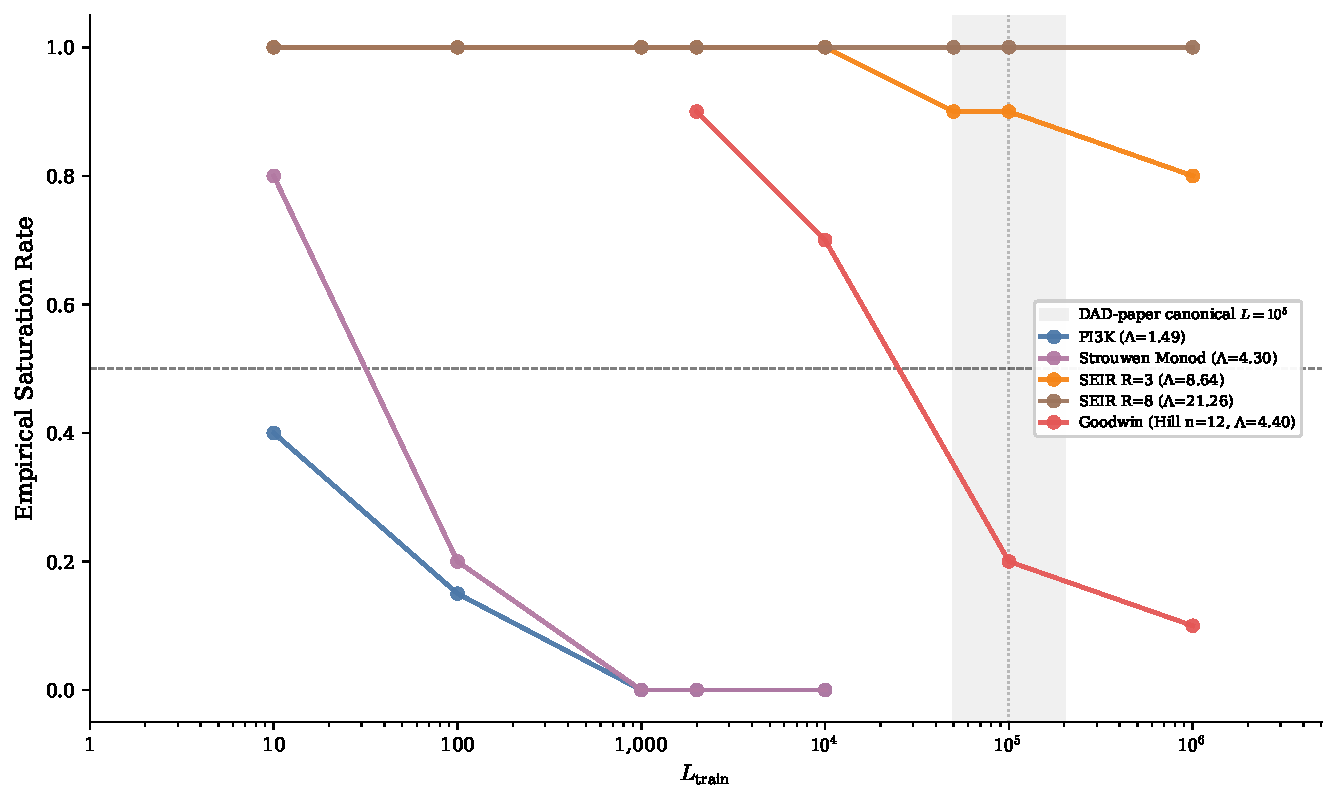
\includegraphics[width=0.78\linewidth]{figures/fig3_lscan_transitions.pdf}
  \caption[Empirical saturation transitions]{Empirical saturation rate against the
  contrastive budget $L$ for five representative systems. PI3K and Monod escape by
  $L\approx30$; the Goodwin oscillator escapes near $L\approx10^4$; SEIR R=3 remains
  at the ceiling across the scan. The shaded band marks the $L=10^5$ budget at which
  policy methods are typically trained.}
  \label{fig:lscan}
\end{figure}

\section{Removing the saturation bias on a controlled toy}
\label{sec:r-toy}

To separate the estimator from the optimiser, we use a controlled six-dimensional
Michaelis-Menten cascade with a prior spanning four orders of magnitude. We sweep the
number of NPE training simulations $N_{\mathrm{NPE}}$ from $10^2$ to $5\times10^4$,
train a fresh posterior estimator in each cell, and evaluate both estimators on
held-out targets at a fixed budget. Figure~\ref{fig:toy} shows the expected phase
transition. The prior-contrastive estimator stays pinned at its ceiling, about six
nats above the true EIG, for every value of $N_{\mathrm{NPE}}$, because no amount of
posterior-estimator training changes where the prior contrastives are drawn from. PACE
descends to the true EIG once the proposal is accurate enough, between
$N_{\mathrm{NPE}}=500$ and $5000$. Since the optimiser is identical in both arms, the
improvement is due to replacing prior contrastives with posterior ones, which is the
core of the cost transfer (RQ2).

\begin{figure}[t]
  \centering
  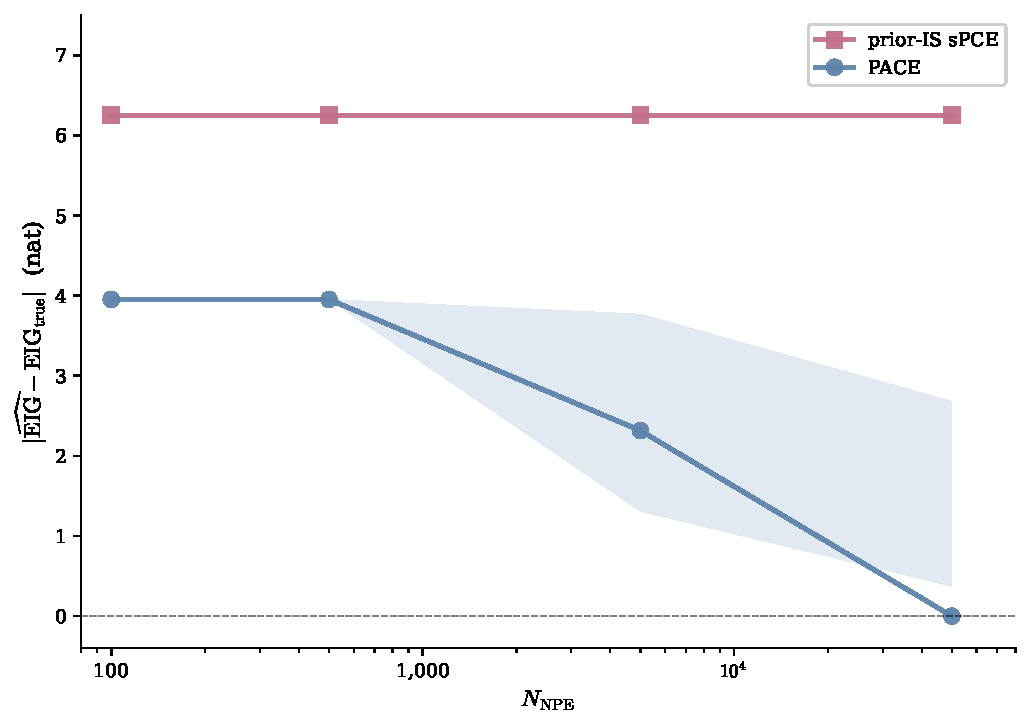
\includegraphics[width=0.6\linewidth]{figures/fig4a_eig_convergence.pdf}
  \caption[Estimator convergence on the controlled toy]{On a six-dimensional
  Michaelis-Menten cascade, PACE converges to the true EIG as the NPE training budget
  $N_{\mathrm{NPE}}$ grows, while the prior-contrastive estimator stays at the
  saturation ceiling regardless of $N_{\mathrm{NPE}}$.}
  \label{fig:toy}
\end{figure}

\section{Anchor systems: where saturation bites}
\label{sec:r-anchors}

Table~\ref{tab:results} is the main comparison against DAD and random design, and
Table~\ref{tab:results-rand} covers the two systems for which no DAD comparator is
available. We read the saturated anchors here and the unsaturated systems in
Section~\ref{sec:r-cross}.

\begin{table}[t]
\centering\footnotesize
\setlength{\tabcolsep}{4pt}
\caption[Per-step EIG bounds: PACE versus DAD and random]{Per-step EIG bounds for
PACE (forward-only), DAD, and random design. Each cell is the mean $\pm$ SEM over $n=300$
rollouts; lower bound ($\uparrow$) is sPCE, upper bound ($\downarrow$) is sNMC.
$\Delta_{\mathrm{sPCE}}$ is the paired PACE${-}$DAD difference $\pm$ SEM with its $t$-test
$p$-value; $\dagger$ marks a definitive ordering. ASM1 and Goodwin are in
Table~\ref{tab:results-rand}.}
\label{tab:results}
\begin{tabular}{lcccccc c}
\toprule
& \multicolumn{2}{c}{PACE} & \multicolumn{2}{c}{DAD} & \multicolumn{2}{c}{Random} & \\
\cmidrule(lr){2-3}\cmidrule(lr){4-5}\cmidrule(lr){6-7}
System ($L_{\mathrm{eval}}$) & Lower bound\,$\uparrow$ & Upper bound\,$\downarrow$ & Lower bound\,$\uparrow$ & Upper bound\,$\downarrow$ & Lower bound\,$\uparrow$ & Upper bound\,$\downarrow$ & $\Delta_{\mathrm{sPCE}}$ ($p$) \\
\midrule
CES ($10^7$)        & $12.98{\pm}0.22$ & $15.37{\pm}0.41$ & $12.05{\pm}0.14$ & $12.17{\pm}0.15$ & $9.01{\pm}0.31$ & $11.11{\pm}0.53$ & $+0.93{\pm}0.18$ ($3.6\mathrm{e}{-}7$)$^\dagger$ \\
SEIR R=3 ($10^7$)   & $14.78{\pm}0.09$ & $16.85{\pm}0.27$ & $7.47{\pm}2.40$ & $9.34{\pm}2.44$ & $14.16{\pm}0.11$ & $15.42{\pm}0.24$ & $+7.31{\pm}2.41$ ($2.6\mathrm{e}{-}3$)$^\dagger$ \\
Monod ($5{\times}10^3$) & $5.28{\pm}0.06$ & $5.35{\pm}0.07$ & $5.94{\pm}0.06$ & $6.07{\pm}0.07$ & $4.77{\pm}0.06$ & $4.81{\pm}0.06$ & $-0.66{\pm}0.07$ ($3.2\mathrm{e}{-}17$)$^\dagger$ \\
\midrule
Src.\ loc.\ $p{=}2$ ($10^5$) & $9.12{\pm}0.11$ & $9.83{\pm}0.18$ & $7.60{\pm}0.11$ & $7.73{\pm}0.13$ & $4.63{\pm}0.12$ & $4.65{\pm}0.12$ & $+1.52{\pm}0.15$ ($3.9\mathrm{e}{-}20$)$^\dagger$ \\
Src.\ loc.\ $p{=}5$ ($10^5$) & $9.84{\pm}0.11$ & $11.89{\pm}0.27$ & $8.77{\pm}0.13$ & $9.42{\pm}0.20$ & $4.19{\pm}0.15$ & $4.22{\pm}0.15$ & $+1.07{\pm}0.18$ ($5.8\mathrm{e}{-}9$)$^\dagger$ \\
Src.\ loc.\ $p{=}8$ ($10^5$) & $5.66{\pm}0.17$ & $5.78{\pm}0.19$ & $5.99{\pm}0.15$ & $6.09{\pm}0.16$ & $1.87{\pm}0.11$ & $1.87{\pm}0.11$ & $-0.34{\pm}0.23$ ($0.15$) \\
PK 1-comp $T{=}3$ ($2$K) & $2.61{\pm}0.08$ & $2.63{\pm}0.09$ & $2.62{\pm}0.08$ & $2.64{\pm}0.08$ & $2.08{\pm}0.16$ & $2.09{\pm}0.16$ & $-0.01{\pm}0.09$ ($0.88$) \\
PK 1-comp $T{=}5$ ($2$K) & $3.25{\pm}0.09$ & $3.29{\pm}0.09$ & $3.19{\pm}0.08$ & $3.23{\pm}0.08$ & $2.76{\pm}0.16$ & $2.77{\pm}0.16$ & $+0.07{\pm}0.09$ ($0.47$) \\
PK 8-comp ($2$K)    & $2.26{\pm}0.07$ & $2.27{\pm}0.07$ & $2.11{\pm}0.07$ & $2.12{\pm}0.07$ & $0.96{\pm}0.06$ & $0.97{\pm}0.06$ & $+0.16{\pm}0.07$ ($0.028$)$^\dagger$ \\
PI3K $T{=}8$ ($10^5$) & $6.37{\pm}0.10$ & $6.45{\pm}0.12$ & $6.52{\pm}0.09$ & $6.55{\pm}0.10$ & $2.45{\pm}0.09$ & $2.45{\pm}0.09$ & $-0.14{\pm}0.10$ ($0.16$) \\
\bottomrule
\end{tabular}
\end{table}

On the saturated systems PACE matches or beats the policy. On CES, PACE's lower bound
($12.98$) exceeds DAD's upper bound ($12.17$), so the ordering is definitive and the
paired gain of $+0.93$ nats cannot be an estimation artifact. On SEIR R=3 the gain is
$+7.31$ nats, but this number must be read carefully: DAD's median rollout is healthy,
and its mean is dragged down by a tail of catastrophic rollouts that PACE does not
produce, which we examine below. Monod is an honest counter-case. Its escape threshold
is small (Table~\ref{tab:escape}), so the policy trains without saturation and wins by
$-0.66$ nats, with both brackets tight enough that the ordering is definitive. PACE
still beats random on Monod ($5.28$ against $4.77$), so the loss is to a better method,
not a failure of the estimator.

\begin{table}[t]
\centering\small
\caption[Systems without a DAD comparator]{Systems where DAD is unavailable. ASM1:
policy training is infeasible (stiff-ODE adjoint, high escape threshold;
Section~\ref{sec:m-forward}). Goodwin: a predicted identifiability counter-case on
which policy training also saturates. Conventions as in Table~\ref{tab:results};
ASM1 uses $n=292$ after excluding non-finite rollouts.}
\label{tab:results-rand}
\begin{tabular}{lcccc c}
\toprule
& \multicolumn{2}{c}{PACE} & \multicolumn{2}{c}{Random} & \\
\cmidrule(lr){2-3}\cmidrule(lr){4-5}
System ($L_{\mathrm{eval}}$) & Lower bound\,$\uparrow$ & Upper bound\,$\downarrow$ & Lower bound\,$\uparrow$ & Upper bound\,$\downarrow$ & $\Delta_{\mathrm{sPCE}}$ ($p$) \\
\midrule
ASM1 ($5{\times}10^4$)   & $10.46{\pm}0.05$ & $21.28{\pm}1.54$ & $9.56{\pm}0.10$ & $14.53{\pm}0.61$ & $+0.89{\pm}0.11$ ($3.1\mathrm{e}{-}15$) \\
Goodwin ($5{\times}10^3$) & $6.07{\pm}0.09$ & $6.87{\pm}0.23$ & $6.55{\pm}0.08$ & $7.58{\pm}0.24$ & $-0.48{\pm}0.04$ ($1.6\mathrm{e}{-}27$) \\
\bottomrule
\end{tabular}
\end{table}

Table~\ref{tab:results-rand} carries the two systems without a DAD comparator. On the
stiff ASM1 wastewater model, where policy training is infeasible, PACE beats random
design by $+0.89$ nats. Goodwin is the predicted counter-case from
Section~\ref{sec:m-failure}: its high Hill exponent creates an identifiability
plateau, so the dominant-particle criterion is flat across designs and PACE loses to
random by $-0.48$ nats. The loss is small and is exactly the failure mode the theory
anticipates, not a general breakdown.

The sNMC upper bounds qualify how far these orderings can be trusted. On Monod the
bracket is tight, with a gap below $0.13$ nats, so the sPCE ordering is essentially
exact. On CES the gap is moderate, but the definitive ordering already places PACE
above DAD. On ASM1 the gap is wide, about eleven nats, which confirms that even
$L_{\mathrm{eval}}=5\times10^4$ is far from resolving the true EIG. Because the ceiling
compresses PACE's more informative rollouts more than random's, the reported $+0.89$
nat advantage on ASM1 is conservative rather than optimistic; we do not claim a larger
number than the bracket supports.

The saturation is also visible in how many rollouts sit at the ceiling. On CES, $76\%$
of PACE rollouts are at the ceiling at $L_{\mathrm{eval}}=10^5$, falling to $41\%$ at
$10^7$ while DAD sits at $4\%$; lifting the budget is what exposes the $+0.93$ nat gap.
On ASM1, $97\%$ of PACE rollouts are pinned at $L=5000$. On SEIR R=3, $97\%$ and $95\%$
of PACE and random rollouts are at the ceiling at $10^5$, falling to $52\%$ and $36\%$
at $10^7$. These percentages explain why a naive comparison at the standard budget
would have reported a tie on systems where a real gap exists.

The clearest result on SEIR R=3 is robustness. Table~\ref{tab:dad-sweep} sweeps DAD
across five training budgets. Its catastrophic-rollout rate, the fraction of rollouts
with sPCE below $-100$ nats, is never zero, is non-monotone in the budget, and is
worst at the largest budget tested. PACE and random produce no catastrophic rollouts
at any budget. The non-monotonicity matters for interpretation: it means the failure
is structural, a consequence of training against a saturated signal, and not something
that more training budget would fix.

\begin{table}[t]
\centering\small
\caption[DAD training sweep on SEIR R=3]{DAD across five training budgets on SEIR R=3,
evaluated at $L_{\mathrm{eval}}=10^5$, $n=300$. The catastrophic rate (rollouts with
sPCE $<-100$ nats) never reaches zero and is highest at the largest budget. PACE and
random produce none at any budget.}
\label{tab:dad-sweep}
\begin{tabular}{lrrrr}
\toprule
$L_{\mathrm{train}}$ & mean sPCE & median & min sPCE & catastrophic \\
\midrule
$10^2$ & $-5.06$ & $11.51$ & $-1192$ & $4.0\%$ \\
$10^3$ & $9.94$ & $11.51$ & $-208$ & $0.7\%$ \\
$10^4$ & $1.84$ & $11.51$ & $-683$ & $2.0\%$ \\
$5{\times}10^4$ & $3.10$ & $11.51$ & $-880$ & $2.0\%$ \\
$10^5$ & $-23.42$ & $11.51$ & $-1313$ & $6.3\%$ \\
\midrule
PACE & $11.45$ & $11.51$ & $7.51$ & $0\%$ \\
random & $11.42$ & $11.51$ & $7.10$ & $0\%$ \\
\bottomrule
\end{tabular}
\end{table}

Figure~\ref{fig:anchors} shows the per-rollout deficit distributions for the two stiff
anchors. On ASM1 the PACE deficits concentrate near zero while random spreads below the
ceiling. On SEIR R=3 the strip plot makes the catastrophic tail of DAD visible
alongside the bulk near the ceiling, which both PACE and random avoid.

\begin{figure}[t]
  \centering
  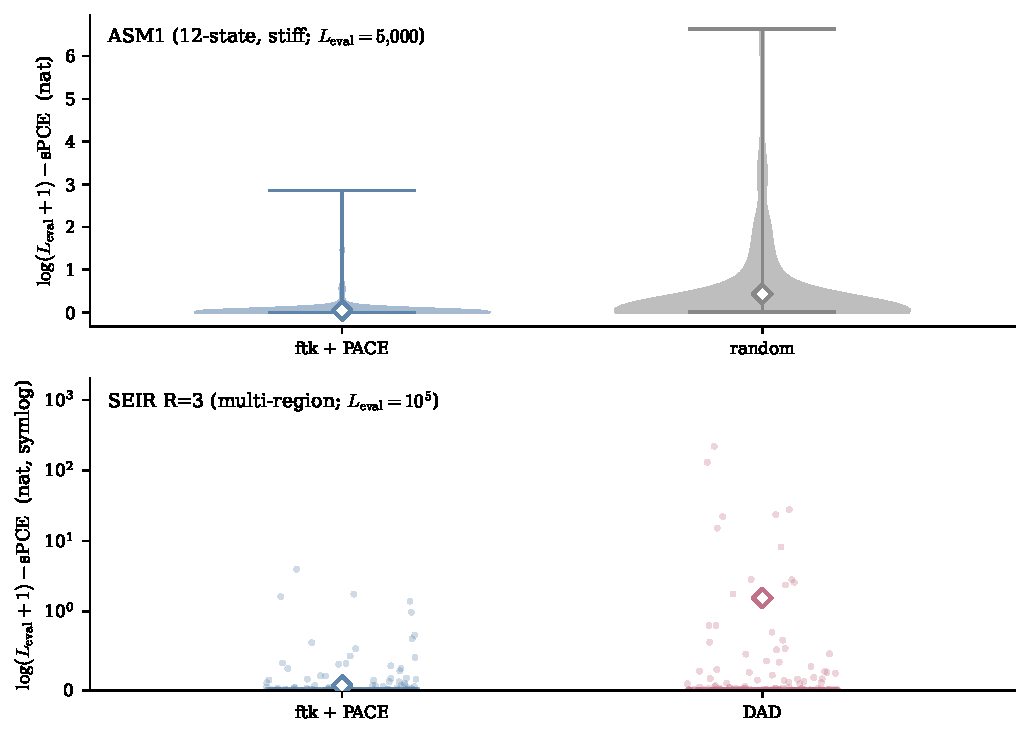
\includegraphics[width=0.6\linewidth]{figures/fig4b_anchors_violin.pdf}
  \caption[Rollout deficits on stiff anchors]{Per-rollout deficit from the evaluation
  ceiling on the stiff anchors, smaller is better. On ASM1 (top) PACE concentrates
  near zero deficit while random spreads below. On SEIR R=3 (bottom) the strip plot
  shows DAD's catastrophic tail, which PACE and random both avoid.}
  \label{fig:anchors}
\end{figure}

\section{Cross-system comparison: where saturation does not bite}
\label{sec:r-cross}

The lower block of Table~\ref{tab:results} covers systems with small escape
thresholds, where the policy trains without saturation and the comparison is
system-specific. PACE wins definitively on source location at $p{=}2$ ($+1.52$) and
$p{=}5$ ($+1.07$) and on the twenty-dimensional PK 8-compartment system ($+0.16$), and
ties DAD on both PK 1-compartment horizons, where the brackets overlap. The policy is
stronger on PI3K ($-0.14$) and on the highest-dimensional source-location task,
$p{=}8$ ($-0.34$). The crossover does not track parameter dimension: PK 8-comp at
$d_\theta=20$ favours PACE while PI3K at $d_\theta=6$ favours DAD. Nor does it track the
effective sample size, as Section~\ref{sec:r-perstep} shows. It tracks whether the
escape threshold exceeds the feasible training budget, which is the screening rule of
Section~\ref{sec:m-saturation}: wherever the threshold is large, PACE matches or beats
the policy. The losses on PI3K and source-location $p{=}8$ are genuine, confirmed by
tight brackets, and we examine in the ablation below whether they are due to the
estimator or the optimiser.

\section{Ablation study}
\label{sec:r-ablation}

The results combine two ingredients, the posterior-contrastive estimator and the
forward-only optimiser. We isolate them in turn. The controlled toy of
Section~\ref{sec:r-toy} already isolated the \emph{estimator}: holding the optimiser
fixed, replacing prior contrastives with posterior ones is what removes the saturation
bias. This section isolates the \emph{optimiser}.

Table~\ref{tab:ablation} compares PACE-grad (Algorithm~\ref{alg:grad}, gradient ascent
on the PACE score) against PACE-ftk (Algorithm~\ref{alg:ftk}, forward-only search) on
the seven systems where both were run. Both variants use the same one-time NPE proposal
and the same candidate budget, so the only difference is the optimiser. With the
proposal held fixed, the optimiser rarely helps and sometimes hurts. Gradient ascent
and forward-only search are statistically indistinguishable on both PK 1-comp horizons,
PK 8-comp, and source location $p{=}5$ ($p\ge0.13$). Gradient ascent helps in exactly
one place, source location $p{=}8$ ($6.27$ against $5.66$, $p=0.003$), where it
reverses the gap with DAD. It hurts on source location $p{=}2$, and most sharply on the
stiff PI3K system, where it loses $0.88$ nats and drops below DAD. On PI3K the adjoint
gradient is uninformative: gradient ascent improves on its random warm start by under
$0.2$ nats, so it reduces to a weaker candidate search than the cross-entropy method
already performs. This is the practical case for the forward-only default. The two
losses to DAD have different causes: on source location $p{=}8$ the optimiser is the
bottleneck and gradient ascent recovers the gap, whereas on PI3K the gradient is the
problem and forward-only search is the better choice.

\begin{table}[t]
\centering\small
\caption[Optimiser ablation]{Optimiser ablation. Both variants use the same one-time
NPE proposal and candidate budget; only the optimiser differs, forward-only
cross-entropy (ftk) versus gradient ascent on the PACE score (grad). Each cell is the
mean $\pm$ SEM over $n=300$ paired rollouts; lower bound ($\uparrow$) is sPCE, upper
bound ($\downarrow$) is sNMC. $\Delta_{\mathrm{sPCE}}$ is the paired grad${-}$ftk
difference $\pm$ SEM. Gradient ascent helps only where the simulator gradient is
reliable and hurts on stiff PI3K.}
\label{tab:ablation}
\begin{tabular}{lcccc c}
\toprule
& \multicolumn{2}{c}{PACE-grad} & \multicolumn{2}{c}{PACE-ftk} & \\
\cmidrule(lr){2-3}\cmidrule(lr){4-5}
System ($L_{\mathrm{eval}}$) & Lower bound\,$\uparrow$ & Upper bound\,$\downarrow$ & Lower bound\,$\uparrow$ & Upper bound\,$\downarrow$ & $\Delta_{\mathrm{sPCE}}$ ($p$) \\
\midrule
Src.\ loc.\ $p{=}2$ ($10^5$) & $8.79{\pm}0.12$ & $9.29{\pm}0.16$ & $9.12{\pm}0.11$ & $9.83{\pm}0.18$ & $-0.33{\pm}0.13$ ($9.4\mathrm{e}{-}3$) \\
Src.\ loc.\ $p{=}5$ ($10^5$) & $10.03{\pm}0.12$ & $12.86{\pm}0.32$ & $9.84{\pm}0.11$ & $11.89{\pm}0.27$ & $+0.19{\pm}0.15$ ($0.20$) \\
Src.\ loc.\ $p{=}8$ ($10^5$) & $6.27{\pm}0.17$ & $6.48{\pm}0.19$ & $5.66{\pm}0.17$ & $5.78{\pm}0.19$ & $+0.61{\pm}0.20$ ($3.1\mathrm{e}{-}3$) \\
PK 1-comp $T{=}3$ ($2$K) & $2.72{\pm}0.08$ & $2.74{\pm}0.08$ & $2.61{\pm}0.08$ & $2.63{\pm}0.09$ & $+0.11{\pm}0.09$ ($0.24$) \\
PK 1-comp $T{=}5$ ($2$K) & $3.23{\pm}0.08$ & $3.27{\pm}0.09$ & $3.25{\pm}0.09$ & $3.29{\pm}0.09$ & $-0.03{\pm}0.10$ ($0.78$) \\
PK 8-comp ($2$K)    & $2.16{\pm}0.07$ & $2.17{\pm}0.07$ & $2.26{\pm}0.07$ & $2.27{\pm}0.07$ & $-0.10{\pm}0.07$ ($0.13$) \\
PI3K $T{=}8$ ($10^5$) & $5.49{\pm}0.12$ & $5.55{\pm}0.13$ & $6.37{\pm}0.10$ & $6.45{\pm}0.12$ & $-0.88{\pm}0.07$ ($6.9\mathrm{e}{-}29$) \\
\bottomrule
\end{tabular}
\end{table}

\section{Per-step information and the effective sample size}
\label{sec:r-perstep}

Reading the rollouts step by step shows that performance follows the information
remaining in the posterior, not the effective sample size of the importance weights.
The per-step increment $\Delta S_t$ decays across steps for every method, which
reflects the contracting posterior, while the effective sample size collapses on a
separate schedule. Figure~\ref{fig:perstep} shows the two side by side on CES and SEIR
R=3. The cumulative per-step information of PACE exceeds random by $+0.5$ to $+5.6$
nats and exceeds DAD on the saturated systems; on CES the
totals are $+13.06$ for PACE against $+12.05$ for DAD and $+9.05$ for random, and on
SEIR R=3 they are $+14.83$ against $+7.46$ and $+14.15$.

\begin{figure}[t]
  \centering
  \begin{subfigure}[b]{0.49\linewidth}\centering
    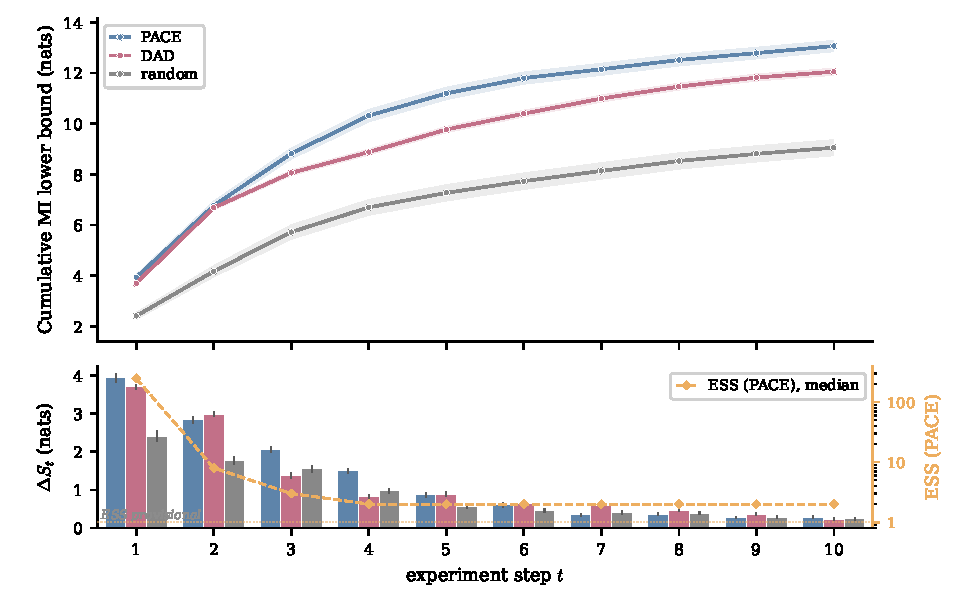
\includegraphics[width=\linewidth]{figures/fig_b7_perstep_eig_ess_CES.pdf}
    \caption{CES}\label{fig:perstep-ces}
  \end{subfigure}\hfill
  \begin{subfigure}[b]{0.49\linewidth}\centering
    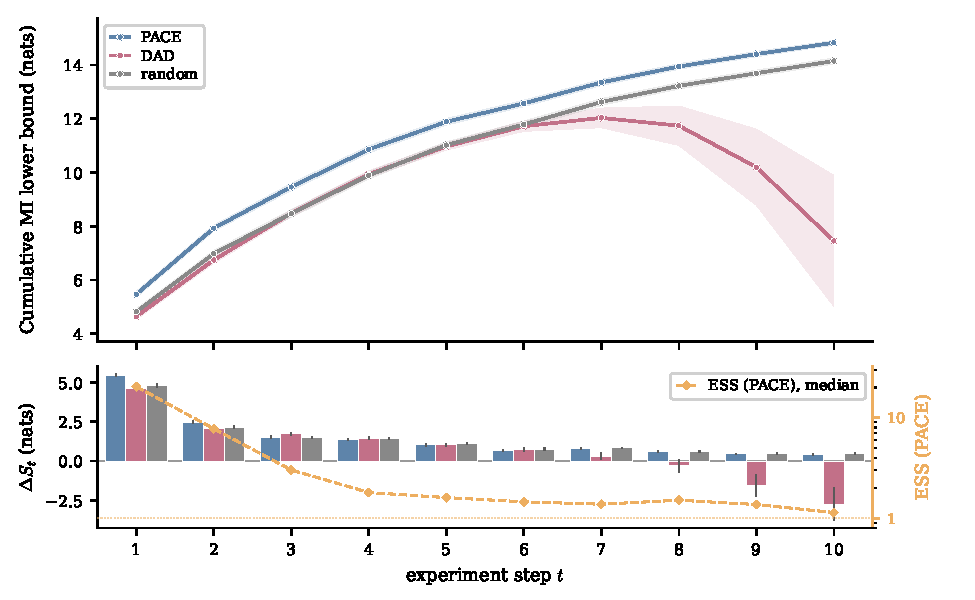
\includegraphics[width=\linewidth]{figures/fig_b7_perstep_eig_ess_SEIR_R_3.pdf}
    \caption{SEIR R=3}\label{fig:perstep-seir}
  \end{subfigure}
  \caption[Per-step information and effective sample size]{Per-step information and
  effective sample size on CES and SEIR R=3. Top of each panel: cumulative information
  for PACE, DAD, and random. Bottom: the per-step increment $\Delta S_t$ as bars, with
  the median PACE effective sample size overlaid (right axis, log scale). The increment
  decays with posterior concentration while the effective sample size collapses on its
  own schedule, yet PACE keeps its lead.}
  \label{fig:perstep}
\end{figure}

Three cases make the disconnect concrete. On SEIR R=3 the effective sample size falls
to one by the final step, yet the per-step gap over DAD grows from $+0.33$ nats in the
first third of the rollout to $+2.02$ nats in the last third, because DAD's late
designs collapse while PACE's stay informative. On CES the effective sample size pins at
about two from the second step onward, yet $70\%$ of PACE's total information is
acquired at an effective sample size of five or below, and the three steps at three or
below alone contribute $34\%$. The cleanest contrast is between PK 8-comp and PI3K. PK
8-comp is the only system that keeps a high effective sample size throughout, at least
$12\%$ of the particle count, yet PACE wins by only $+0.16$ nats; PI3K collapses to
about two like the others, yet also favours DAD by $-0.14$ nats. Neither retaining nor
losing the effective sample size fixes the sign of the gap. For this reason we do not
report a single cross-system correlation between the effective sample size and
performance: the sign of such a fit is not stable across summaries of the same
rollouts. The per-step view is the honest one, and it says performance is set by
whether the policy training signal is saturated, not by whether the importance weights
are degenerate. The full per-step and effective-sample-size tables are in
Appendix~\ref{app:supp}.

\section{Diagnostics: trusting the results under weight collapse}
\label{sec:r-diag}

A collapsing effective sample size looks alarming, so each diagnostic below rules out a
specific failure. The starting point is the identity of Eq.~\eqref{eq:widentity}: a
perfect proposal keeps the effective sample size at its maximum at any concentration,
so a collapse implies a small proposal mismatch amplified by concentration, not a
broken proposal. Four diagnostics confirm this.

First, the chosen design survives resampling. On ASM1, resampling the particle bank two
hundred times at several steps gives a median top-1 agreement of $45\%$ on which design
is selected, about twenty-three times the chance rate of one in fifty candidates. The
common-mode cancellation of Section~\ref{sec:m-cancellation} therefore preserves a
strong directional signal even when the weights have collapsed.

Second, the breakage is in the resampling, not the proposal. Table~\ref{tab:coverage}
separates the two. The coverage of the true parameter by the raw NPE samples, before
importance reweighting, stays between $76\%$ and $90\%$ through the final step on every
system. The coverage after importance resampling collapses, to $36\%$ on PI3K and
$32\%$ on CES at the last step, because resampling from degenerate weights shrinks the
credible set to almost a point. The proposal stays well calibrated; the collapse is a
resampling artifact.

\begin{table}[t]
\centering\small
\caption[Raw versus resampled coverage]{Per-step coverage of the true parameter at the
$90\%$ level, as a fraction of parameter dimensions. Raw is computed on NPE samples
before reweighting and tests the proposal directly; IS is computed after importance
resampling. ESS is the per-step median. Raw coverage stays high while IS coverage
collapses at late steps, isolating the resampling artifact.}
\label{tab:coverage}
\begin{tabular}{lccrcc}
\toprule
System & $d_\theta$ & step & ESS & raw @90\% & IS @90\% \\
\midrule
PK 8-comp & 20 & 1 & 233 & 90\% & 89\% \\
          &    & 5 & 125 & 90\% & 88\% \\
\cmidrule(l){1-6}
PI3K & 6 & 1 & 561 & 90\% & 90\% \\
     &   & 4 & 17 & 85\% & 80\% \\
     &   & 8 & 1.6 & 76\% & 36\% \\
\cmidrule(l){1-6}
CES & 4 & 1 & 8.6 & 88\% & 63\% \\
    &   & 5 & 2.6 & 85\% & 36\% \\
    &   & 10 & 1.7 & 84\% & 32\% \\
\cmidrule(l){1-6}
ASM1 & 12 & 1 & 77 & 90\% & 85\% \\
     &    & 3 & 5.7 & 87\% & 65\% \\
     &    & 5 & 2.7 & 87\% & 50\% \\
\bottomrule
\end{tabular}
\end{table}

Third, calibration is stable across steps. Simulation-based calibration on the raw NPE
samples gives a KS distance between $0.13$ and $0.18$ across systems, flat or improving
across steps, including on CES and ASM1 where the effective sample size falls below ten.
The same diagnostic on resampled samples degrades, which again points to a resampling
artifact rather than a proposal failure. The subtlety here is that calibration on
average, which is what simulation-based calibration tests, is not the same as
calibration at the specific histories where the effective sample size collapses. The
raw coverage in Table~\ref{tab:coverage}, measured at the deployment histories, is the
complementary conditional evidence; both are developed in Appendix~\ref{app:diagnostics}.

Fourth, there is no mode collapse. Gross mode collapse would show as Pareto shapes of
the weights diverging and raw coverage going to zero. Neither occurs: raw coverage
stays at or above $76\%$ and the calibration distances stay small. The method also
moves across more than a hundredfold in effective sample size across systems without
any threshold or mode switch, from the high-coverage multi-particle regime of PK 8-comp
to the single-particle regime of CES and ASM1, which confirms the smooth interpolation
of Section~\ref{sec:m-cancellation}. Together these diagnostics support the central
empirical claim of RQ3: PACE's design rankings are reliable even when its weights have
collapsed.

\section{Computational cost and the budget trade-off}
\label{sec:r-budget}

The cost transfer of Section~\ref{sec:m-pace} is the empirical counterpart of
contribution~2: PACE moves the per-step contrastive cost of policy training onto a
one-time inference pass plus a constant per-step search. This section collects the
budget evidence.

\paragraph{The two cost structures.} A policy trained on the sPCE objective pays, per
gradient step, $L_{\mathrm{train}}$ forward-plus-backward simulator solves, and on
saturated systems $L_{\mathrm{train}}$ must reach $L_{\mathrm{escape},50}$ before the
gradient carries signal (Section~\ref{sec:m-saturation}); the training cost scales as
$O(N_{\mathrm{iter}}\,L_{\mathrm{escape},50}\,T)$. PACE pays a one-time NPE training pass
plus, per step, $J(1+M(1+C)N_{\mathrm{cand}})$ forward-only solves
(Section~\ref{sec:m-forward}). The first grows exponentially with the information per
experiment; the second does not.

\paragraph{Measured costs.} Table~\ref{tab:walltime} reports the numbers. PACE's one-time
NPE training takes $3.6$ to $12.8$ minutes across the suite, and generating that training
data takes under a minute on the non-stiff systems and $5$ to $60$ minutes on the stiff
ones. At deployment PACE selects each design in under four seconds on eleven of twelve
systems, the exception being the stiff ASM1 model at $40.5$\,s. Policy training, by
contrast, ranges from about seven minutes on the simplest systems to sixteen hours on
Monod, is unstable on CES, and is infeasible on ASM1 and on SEIR R=3 at the budget needed
to escape saturation. A deployed policy then emits designs in milliseconds, faster than
PACE per step, but this latency gap is irrelevant for scientific experiments that take
minutes to weeks to run; the decisive comparison is the one-time training cost.

\paragraph{Budget versus quality.} Two results bound the trade-off. The cost-shift toy
(Figure~\ref{fig:toy}) sets the lower end: PACE reaches the true EIG once its NPE is
trained on only $500$ to $5000$ simulations, while the prior-contrastive estimator stays
pinned regardless of budget. The DAD L-sweep (Table~\ref{tab:dad-sweep}) sets the other
end: on SEIR R=3 the policy never escapes saturation across five orders of magnitude of
$L_{\mathrm{train}}$, so no feasible policy budget buys a usable design. Together they
make the cost transfer concrete: PACE's budget is bounded and paid once, whereas the
policy's required budget is unbounded on exactly the systems where design matters most.
% TODO(planned sweeps -- see PLANNED_EXPERIMENTS.md):
% A1 real-anchor N_NPE sweep (CES/SEIR) -> figure generalising the toy phase transition;
% A2 quality/cost vs particle count J; A3 quality vs CEM budget (N_cand, C).
% Drop figures/tables and a sentence here once the runs are complete.
